%!TEX root = ../thesis-main.tex
\chapter{Design}

Alchemist, come esplicato nella sezione \ref{sec:alchemist}, è un software modulare complesso in continuo sviluppo, gli strumenti presentati nel capitolo precedente trovano già impiego nel progetto, ad eccezione del software di impacchettamento il quale è oggetto di questo elaborato. Di seguito sarà illustrata l'architettura e l'interazione tra i componenti principali che compaiono nel processo di automazione.

\section{Architettura e macrostruttura}

L'analisi del progetto espone il coinvolgimento di tre diversi componenti per conseguire gli obiettivi di automazione e distribuzione del software. I tre componenti sono definiti come segue: 
\begin{itemize}
	\item \textbf{Pipeline}: il processo automatizzato adibito alla gestione del flusso di lavoro del software, dalla compilazione al rilascio. Questo componente è già impiegato all'interno del progetto Alchemist per gestire l'attuale processo di integrazione continua, il design discusso in questo capitolo inserisce nuovi step all'interno del processo.
	\item \textbf{Build system}: l'insieme dei processi e delle funzioni adibite alla produzione di artefatti. In particolare questo componente richiede lo sviluppo di nuovi processi destinati alla produzione dei pacchetti, test di quest'ultimi e costruzione dei metadati necessari al rilascio del software.
	\item \textbf{Release}: i processi necessari e le regole vigenti per la pubblicazione del software nei repository pubblici.
\end{itemize}
I componenti interagiscono come raffigurato nella figura \ref{fig:activity-interaction-diagram} La pipeline sfrutta il build system per generare i pacchetti di installazione del software e integra tutti i processi necessari alla distribuzione negli specifici repository pubblici, producendo quindi l'automazione desiderata.

\begin{figure}[H]
	\centering
	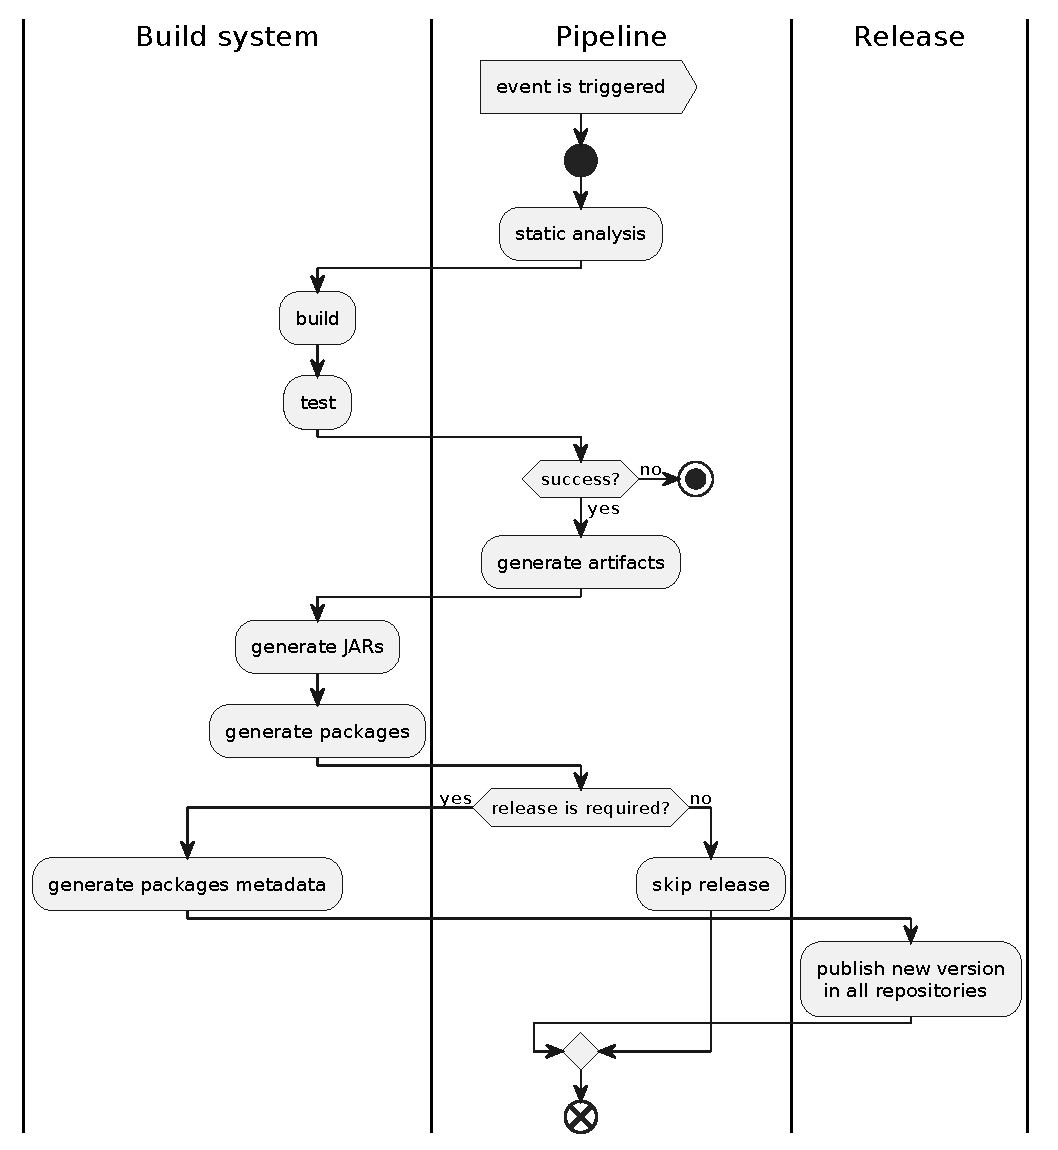
\includegraphics[width=.9\linewidth]{figures/activity-interaction-diagram.pdf}
	\caption{Diagramma delle attività raffigurante l'interazione tra i componenti}
	\label{fig:activity-interaction-diagram}
\end{figure}

Nello schema si fa riferimento ad un generico \texttt{evento} come segnale di inizio della pipeline. Nell'ambito \ac{cicd} l'evento corrisponde spesso alla pubblicazione di nuovo codice nel repository, di modo che ad ogni aggiunta la pipeline restituisce un feedback positivo o negativo e lo sviluppatore può agire di conseguenza.

\section{Pipeline}

Alchemist utilizza fondamentalmente due workflow per soddisfare i requisiti di integrazione e rilascio continuo. Un primo workflow chiamato ``dispatcher", il quale funziona come punto di inizio del flusso, è in ascolto di eventi e una volta avviato esamina i meta-dati dell'evento scatenante per determinare il flusso successivo. In particolare nella configurazione in oggetto questo step iniziale funge da filtro dal momento che esiste un solo possibile flusso successivo, ossia il secondo workflow quello adibito a soddisfare i compiti di build, test e distribuzione.
Per compiere le tre funzioni il workflow è formato dai seguenti job.
\begin{itemize}
	\item \textbf{select-java-version}: è il punto di inizio ed ha il compito di propagare la versione minima supportata per replicare lo stesso ambiente \ac{jre} nei successivi job.
	\item \textbf{build}: esegue un'analisi statica del codice e gli unit test. Utilizza una strategia a matrice per costruire più istanze in ambienti diversi: in questo caso nei tre sistemi operativi principali. 
	\item \textbf{test-deploy}: esegue un test del deploy dei moduli di Alchemist. Il test è strettamente necessario per l'esecuzione corretta di un rilascio.
	\item \textbf{build-website}: costruisce il sito web di documentazione e lo prepara per il rilascio.
	\item \textbf{release}: analizza attraverso tecniche di semantic-versioning se è necessario il rilascio di una nuova versione del software. In caso positivo: costruisce i JAR, ottiene il sito e pubblica una nuova versione.
	\item \textbf{success}: infine, controlla che l'output di ogni job sia esente da errori.
\end{itemize}

\subsection{Workflow risultante} La nuova pipeline, descritta in figura 3.2, introduce due job all'interno del flusso cercando di sfruttare il più possibile la computazione parallela per ottimizzare i tempi di esecuzione.
\begin{figure}[H]
	\centering
	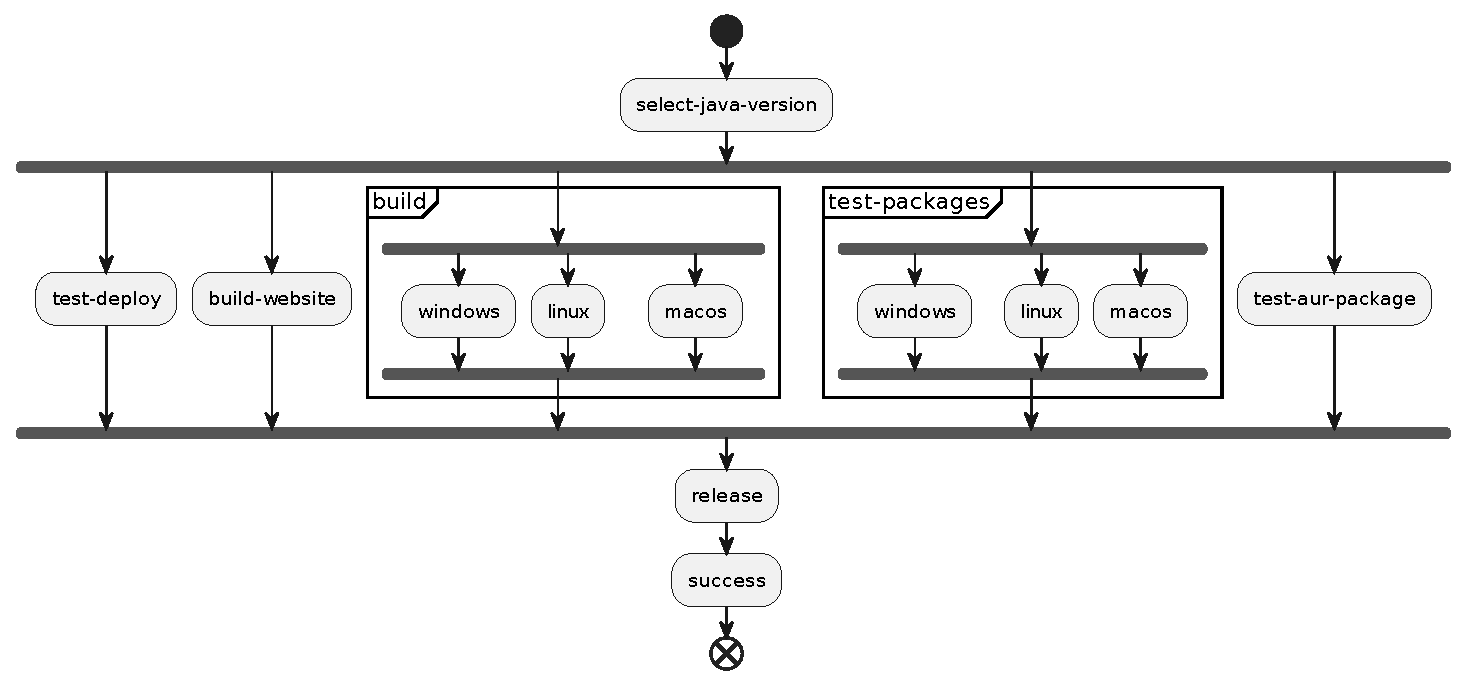
\includegraphics[width=1\linewidth]{figures/activity-diagram-pipeline.pdf}
	\caption{Diagramma dell'attività illustrante la pipeline}
	\label{fig:activity-diagram-pipeline}
\end{figure}
Mentre per la generazione ed il rilascio esistono già dei job adibiti, è buona norma configurare singoli job riservati al test di una particolare funzionalità, in modo che il test venga eseguito in un ambiente basilare senza potenziali modifiche che possono interferire con l'esito. Il comportamento di default dei job all'interno della pipeline è bloccante per cui il fallimento di un test porta all'interruzione dell'intera pipeline.

\begin{figure}[H]
	\centering
	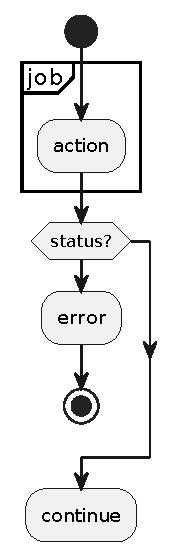
\includegraphics[width=.13\linewidth]{figures/activity-diagram-job.pdf}
	\caption{Diagramma dell'attività illustrante il comportamento dei job all'interno della pipeline}
	\label{fig:activity-diagram-job}
\end{figure}

Il primo job \texttt{test-packages} utilizza la strategia a matrice per eseguire la procedura sui tre sistemi operativi target del progetto ed ha il compito di generare e controllare la validità dei pacchetti di installazione. Il secondo \texttt{test-aur-package} installa localmente il pacchetto all'interno di un container \textit{arch-linux}, infine controlla il corretto esito dell'operazione costruendo il pacchetto con \textit{makepkg} ed installandolo con \textit{pacman}.

\section{Build system}

Il ruolo principale del \textit{build system} è quello di esporre un \textit{task} adibito alla generazione dei pacchetti. Il task dovrà soddisfare i seguenti requisiti:
\begin{itemize}
	\item Deve configurare correttamente le opzioni di \textit{jpackage}, in particolare quelle che mutano nel tempo come la versione.
	\item È necessario stabilire un corretto ordine di esecuzione ed albero delle dipendenze per garantire la consistenza del processo.
	\item Deve consentire la dichiarazione di configurazioni differenti a seconda del sistema operativo che esegue il processo.
\end{itemize}

\subsection{JPackage} Lo strumento \ac{cli} \textit{jpackage} offre un'interfaccia munita di diverse opzioni per configurare e personalizzare a piacimento i pacchetti in output. Esistono parametri generici, compatibili con tutte le piattaforme, e parametri specifici che vanno a modificare attributi particolari alla tipologia di pacchetto in output scelta. Uno dei motivi che ha portato alla scelta di \textit{jpackage} rispetto ad altri software è la capacità di includere autonomamente una \textit{runtime-image} di Java, ossia una \ac{jre} ridotta di dimensioni all'interno del pacchetto. La combinazione di una \textit{runtime-image} e degli archivi Java (JAR) necessari all'esecuzione dell'applicazione costituiscono l'\textit{application-image}: un pacchetto autocontenuto che include l'applicazione, assieme una \ac{jvm} ed alle librerie necessarie per eseguire quell'applicazione sulla piattaforma di destinazione.

Alchemist è un progetto modulare ed ogni modulo è distribuito in un archivio JAR specifico. Come descritto nella documentazione\footnote{https://alchemistsimulator.github.io/howtos/preparation/jar/index.html} il software predispone due modalità di utilizzo stand-alone attraverso l'esecuzione degli archivi Java. La prima modalità consiste nell'inclusione dei singoli moduli richiesti come \textit{classpath} del processo di esecuzione. La seconda modalità sfrutta l'archivio denominato ``full", ossia un \textit{fat-jar} contenente tutti i moduli e tutte le dipendenze necessarie all'esecuzione del software in tutte le sue parti. In ottica di ridurre le dimensioni del pacchetto e velocizzare il processo di impacchettamento, jpackage costruirà l'\textit{application-image} utilizzando quest'ultimo. La posizione ed organizzazione dei file è diversa a seconda della piattaforma di destinazione del pacchetto, il risultato dell'installazione in un ambiente Linux è descritto nella figura 3.3.  

\begin{figure}
	\centering
	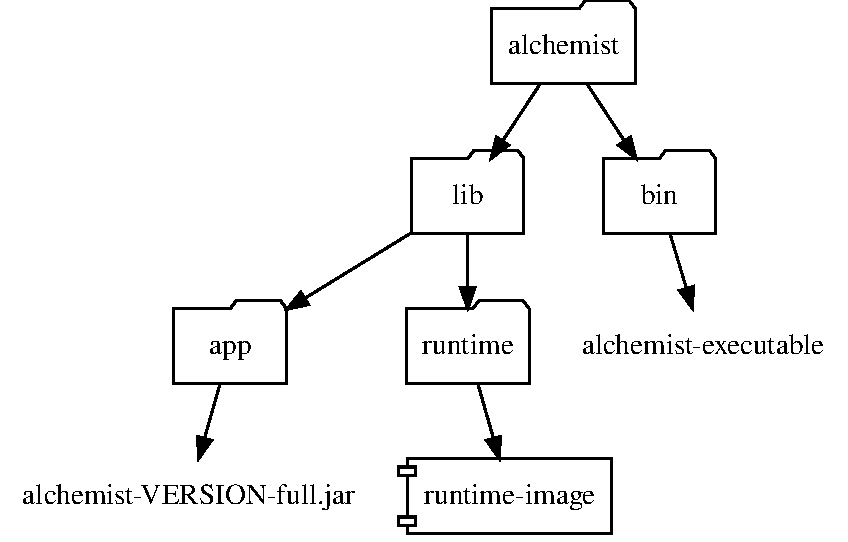
\includegraphics[width=.7\linewidth]{figures/application-image-folder-structure.pdf}
	\caption{Struttura del filesystem dell'\textit{application image} generato da \textit{jpackage} con Linux come piattaforma target}
	\label{fig:application-image-folder-structure}
\end{figure}

Per introdurre jpackage nel build system è necessario un task che funga da \textit{wrapper}: il quale esponga proprietà corrispondenti alle opzioni della \ac{cli} di jpackage. Gradle utilizza una pratica denominata \textit{lazy configuration} che fornisce la dichiarazione delle \textit{lazy properties} vale a dire ``proprietà pigre". Questa caratteristica consente di legare una proprietà ad un'altra senza doversi preoccupare dell'ordine di esecuzione. In tale modo non sono necessarie particolari attenzioni nell'assegnazione di proprietà come la versione, la quale viene calcolata da un plugin apposito.

Il programma jpackage, come illustrato nella sezione \ref{ssec:packaging}, non è \textit{cross-platform}, ciò significa che la generazione dei pacchetti deve essere eseguita su un dispositivo ospitante il sistema operativo di destinazione dei pacchetti richiesti. Per quanto lo strumento cerchi di unificare i diversi ambienti, ogni tipologia di pacchetto specialmente se di piattaforme diverse presenta limiti e regole differenti. Per questa ragione il task deve prevedere l'utilizzo di valori differenti a seconda del sistema operativo sottostante.

\subsection{Design risultante}  

\begin{figure}
	\centering
	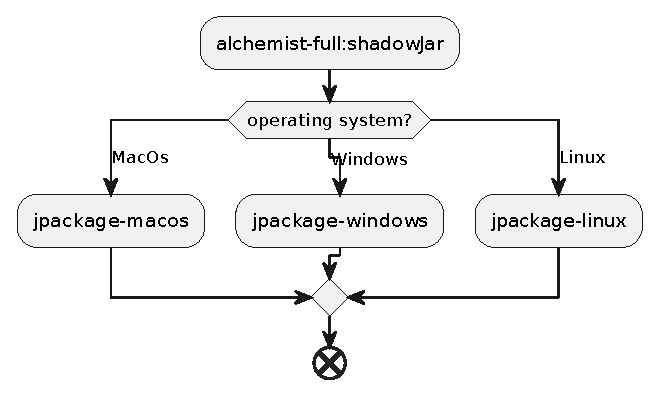
\includegraphics[width=.8\linewidth]{figures/gradle-jpackage-scheme.pdf}
	\caption{Diagramma delle attività rappresentante il processo di generazione dei pacchetti}
	\label{fig:gradle-jpackage-scheme}
\end{figure}

\section{Release}

\subsection{Repository}

\paragraph{AUR}

\paragraph{WinGet}

\paragraph{Snapcraft e Flathub}

\subsection{Conclusioni e punti comuni}
